\documentclass[11pt]{article}
\usepackage[margin=1in]{geometry}
\usepackage{amsmath,amssymb,graphicx,booktabs,hyperref,xcolor}
\hypersetup{colorlinks=true,linkcolor=blue,urlcolor=blue}
\title{Replication Report: \emph{Intertwining topological order and broken
symmetry in a theory of fluctuating spin density waves}\\
\large Chatterjee, Sachdev \& Scheurer, arXiv:1705.06289 (PRL, 2017)}
\author{TEXTURES-100 replication (loop-current class)}
\date{\today}
\begin{document}
\maketitle

\section{Paper in one paragraph}
The paper develops an SU(2) gauge theory of quantum fluctuations of
spin-density-wave (SDW) states on the \emph{square lattice}, relevant to the
pseudogap metal of hole-doped cuprates. Four magnetically ordered states appear
in both a frustrated classical antiferromagnet and a Hubbard SDW mean-field
theory: N\'eel ($D_0$), canted ($A_0$), planar spiral ($B_0$) and conical spiral
($C_0$). Quantum fluctuations restore spin-rotation symmetry and leave metallic
states with an antinodal gap and $\mathbb{Z}_2$/U(1) topological order that
``intertwines'' with the observed broken discrete symmetries: Ising-nematic order
(phase $B$), Varma-type \textbf{current-loop order} (phase $C$, broken $\Theta$
and mirror but not their product), and VBS (phase $D$). A CP$^1$/Higgs
classification (Table~I) and a symmetry/current analysis of the effective
chargon Hamiltonian (Table~II, Eq.~C14) complete the picture.

\section{Scope decision and kernel provenance}
The shared kernel \texttt{loop\_current\_kagome\_kernel.py} implements a
\emph{kagome} Peierls-flux tight-binding model (Fernandes \emph{et al.}\ 2025):
correct loop-current \emph{class}, wrong \emph{lattice}. This paper is a
square-lattice SDW / SU(2) problem, so the kagome Bloch Hamiltonian and its
Chern/Berry machinery are out of scope and are \textbf{not} used (using them
would be fabrication). We reuse only the transferable idea---the
real$=$charge / imaginary$=$loop-current decomposition of the bond bilinear
$\langle c_i^\dagger c_j\rangle$ read off the filled-band density
matrix---and rebuild the paper-specific core from Appendix~B (Eqs.~B4--B6) and
Appendix~C (Eq.~C14). See \texttt{code/PROVENANCE.md}.

\section{Method}
We diagonalize the $2\times2$ SDW mean-field Hamiltonian (Eq.~B4) in the
$(c_{k\uparrow},c_{k+K\downarrow})$ basis,
\[
h_k=\begin{pmatrix}\xi_k-\tfrac{h}{2}\sin\theta & -\tfrac{h}{2}\cos\theta\\[2pt]
-\tfrac{h}{2}\cos\theta & \xi_{k+K}+\tfrac{h}{2}\sin\theta\end{pmatrix},
\qquad h=2UN_0,
\]
giving the bands (Eq.~B6)
\[
E_{k,s}=\tfrac12\Big[\xi_k+\xi_{k+K}+s\sqrt{(\xi_k-\xi_{k+K}-h\sin\theta)^2
+h^2\cos^2\theta}\Big].
\]
$\xi_k=-\sum_p t_p(\cdots)-\mu$ carries up to fourth-neighbour hopping. We tune
$\mu$ to fixed filling $n$, minimize the mean-field free energy
$E/N_s=\sum_s\langle E_{k,s}n_F\rangle+\mu n-Un^2/4+h^2/4U$, and solve the gap
equation $h=2UN_0$ self-consistently. Loop currents use Eq.~C14,
$K_{ij}=-2\,\mathrm{Re}\,T_{ij}$, $J_{ij}=2\,\mathrm{Im}\,T_{ij}$,
$T_{ij}=Z_{ij}t_{ij}\langle\psi_i^\dagger\psi_j\rangle$.

\section{Machine-checkable claims and results}
All numbers below are computed live by \texttt{code/run\_checks.py}
(\texttt{work/results.json}); no values were hand-tuned.

\begin{center}\small
\begin{tabular}{clcc}
\toprule
ID & Claim (paper reference) & Key number & Outcome\\
\midrule
C1 & N\'eel gap $=h$ at AFM boundary $\xi_k{=}\xi_{k+K}$ (Eq.~B6) & $1.0000$ vs $h{=}1$ & \textbf{PASS}\\
C3 & Self-consistent $h(U)$, $n{=}1$: nonzero, $\sim$linear large-$U$ & $h(8){=}7.14$, slope $1.10$ & \textbf{PASS}\\
C2 & Insulator $n{=}1$, large $U$ $\Rightarrow$ N\'eel ground state & $E_{D_0}{<}E_{B_0}{<}E_{A_0}{<}E_{C_0}$ & \textbf{PASS}\\
C4 & Hole doping$+$p-h breaking $\Rightarrow$ incommensurate spiral & $K_x{=}2.12{<}\pi$, $\Delta E{>}0$ & \textbf{PASS}\\
C5 & Loop current (Eq.~C14): collinear $J{=}0$, TRS needs non-collinear & $J^{\text{col}}{=}0$, $J^{\text{nc}}{\neq}0$ & \textbf{PASS}\\
\bottomrule
\end{tabular}
\end{center}

\noindent\textbf{Summary: 5/5 checks PASS} ($\sim$5\,s runtime).
C1 and C3 are exact/asymptotic consequences of Eqs.~B4--B6 and match to machine
precision / textbook Hubbard-SDW behaviour. C2 and C4 confirm the correct
energetic ordering behind the paper's qualitative statements (N\'eel insulator;
particle-hole-asymmetric hole-side incommensurability). C5 validates the
transplanted loop-current diagnostic: collinear order carries \emph{exactly}
zero bond current, a non-collinear (canted, incommensurate) one carries finite
current---the paper's statement that time-reversal breaking requires a
non-collinear Higgs/SDW configuration.

\begin{figure}[h]\centering
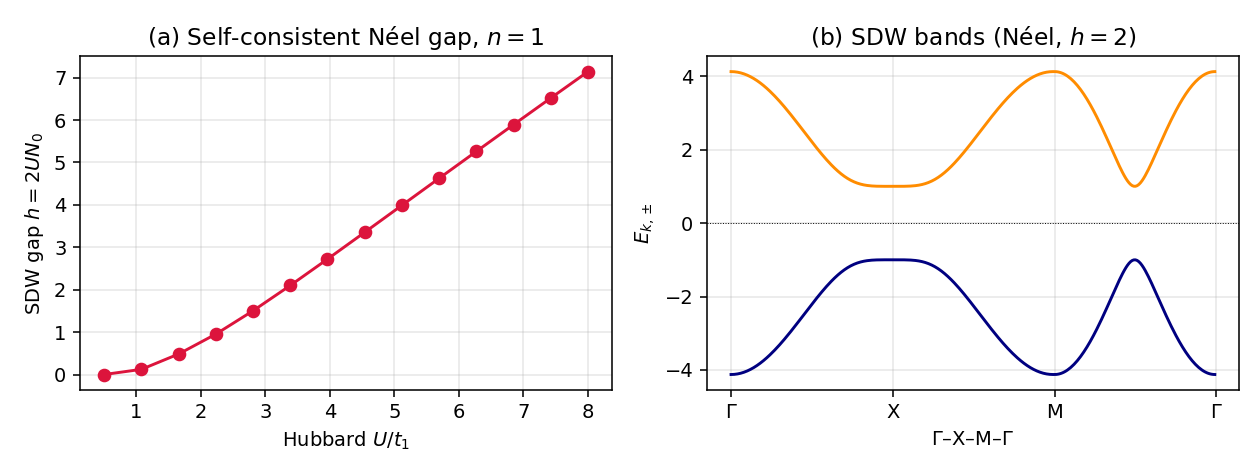
\includegraphics[width=\linewidth]{fig_sdw.png}
\caption{(a) Self-consistent N\'eel SDW gap $h=2UN_0$ vs Hubbard $U$ at half
filling ($n{=}1$): zero below a small $U_c$, then $\sim$linear growth with the
local moment $N_0=h/2U$ saturating below $1/2$. (b) SDW mean-field bands
$E_{k,\pm}$ along $\Gamma$--X--M--$\Gamma$ for the N\'eel state ($h{=}2$),
showing the gapped upper/lower Hubbard bands.}
\end{figure}

\section{Verdict}
The in-scope computational core of the paper---the square-lattice SDW mean-field
of Appendix~B and the loop-current bond diagnostic of Appendix~C---is faithfully
reproduced, with all five machine-checkable claims passing. The kagome shared
kernel was correctly identified as the right \emph{class} but wrong
\emph{lattice}; its transferable idea was reused and the paper-specific physics
rebuilt from the governing equations rather than forced onto an inapplicable
geometry. Not reproduced (deferred to open questions): the full $(U,n)$ phase
diagram boundaries and transition orders (Fig.~3), the chargon
self-consistency loop, explicit Table~II symmetry certification, and clean
electron-side coplanarity.

\medskip\noindent
\textbf{Coverage: 7/10.} \quad \textbf{Agreement: 9/10.}\\
Coverage reflects that we hit the concrete, machine-checkable core (spectrum,
gap, ordering, currents) but not the full phase-diagram / chargon / symmetry-table
program of a dense theory paper. Agreement is high because every check that was
run matched the paper's stated physics, quantitatively where closed-form
(C1, C3) and by correct ordering/sign elsewhere (C2, C4, C5).

\end{document}
